% Options for packages loaded elsewhere
\PassOptionsToPackage{unicode}{hyperref}
\PassOptionsToPackage{hyphens}{url}
%
\documentclass[
]{book}
\usepackage{lmodern}
\usepackage{amssymb,amsmath}
\usepackage{ifxetex,ifluatex}
\ifnum 0\ifxetex 1\fi\ifluatex 1\fi=0 % if pdftex
  \usepackage[T1]{fontenc}
  \usepackage[utf8]{inputenc}
  \usepackage{textcomp} % provide euro and other symbols
\else % if luatex or xetex
  \usepackage{unicode-math}
  \defaultfontfeatures{Scale=MatchLowercase}
  \defaultfontfeatures[\rmfamily]{Ligatures=TeX,Scale=1}
\fi
% Use upquote if available, for straight quotes in verbatim environments
\IfFileExists{upquote.sty}{\usepackage{upquote}}{}
\IfFileExists{microtype.sty}{% use microtype if available
  \usepackage[]{microtype}
  \UseMicrotypeSet[protrusion]{basicmath} % disable protrusion for tt fonts
}{}
\makeatletter
\@ifundefined{KOMAClassName}{% if non-KOMA class
  \IfFileExists{parskip.sty}{%
    \usepackage{parskip}
  }{% else
    \setlength{\parindent}{0pt}
    \setlength{\parskip}{6pt plus 2pt minus 1pt}}
}{% if KOMA class
  \KOMAoptions{parskip=half}}
\makeatother
\usepackage{xcolor}
\IfFileExists{xurl.sty}{\usepackage{xurl}}{} % add URL line breaks if available
\IfFileExists{bookmark.sty}{\usepackage{bookmark}}{\usepackage{hyperref}}
\hypersetup{
  pdftitle={Modul Praktikum Statistika dengan R},
  pdfauthor={I Made Krisna Gupta},
  hidelinks,
  pdfcreator={LaTeX via pandoc}}
\urlstyle{same} % disable monospaced font for URLs
\usepackage{color}
\usepackage{fancyvrb}
\newcommand{\VerbBar}{|}
\newcommand{\VERB}{\Verb[commandchars=\\\{\}]}
\DefineVerbatimEnvironment{Highlighting}{Verbatim}{commandchars=\\\{\}}
% Add ',fontsize=\small' for more characters per line
\usepackage{framed}
\definecolor{shadecolor}{RGB}{248,248,248}
\newenvironment{Shaded}{\begin{snugshade}}{\end{snugshade}}
\newcommand{\AlertTok}[1]{\textcolor[rgb]{0.94,0.16,0.16}{#1}}
\newcommand{\AnnotationTok}[1]{\textcolor[rgb]{0.56,0.35,0.01}{\textbf{\textit{#1}}}}
\newcommand{\AttributeTok}[1]{\textcolor[rgb]{0.77,0.63,0.00}{#1}}
\newcommand{\BaseNTok}[1]{\textcolor[rgb]{0.00,0.00,0.81}{#1}}
\newcommand{\BuiltInTok}[1]{#1}
\newcommand{\CharTok}[1]{\textcolor[rgb]{0.31,0.60,0.02}{#1}}
\newcommand{\CommentTok}[1]{\textcolor[rgb]{0.56,0.35,0.01}{\textit{#1}}}
\newcommand{\CommentVarTok}[1]{\textcolor[rgb]{0.56,0.35,0.01}{\textbf{\textit{#1}}}}
\newcommand{\ConstantTok}[1]{\textcolor[rgb]{0.00,0.00,0.00}{#1}}
\newcommand{\ControlFlowTok}[1]{\textcolor[rgb]{0.13,0.29,0.53}{\textbf{#1}}}
\newcommand{\DataTypeTok}[1]{\textcolor[rgb]{0.13,0.29,0.53}{#1}}
\newcommand{\DecValTok}[1]{\textcolor[rgb]{0.00,0.00,0.81}{#1}}
\newcommand{\DocumentationTok}[1]{\textcolor[rgb]{0.56,0.35,0.01}{\textbf{\textit{#1}}}}
\newcommand{\ErrorTok}[1]{\textcolor[rgb]{0.64,0.00,0.00}{\textbf{#1}}}
\newcommand{\ExtensionTok}[1]{#1}
\newcommand{\FloatTok}[1]{\textcolor[rgb]{0.00,0.00,0.81}{#1}}
\newcommand{\FunctionTok}[1]{\textcolor[rgb]{0.00,0.00,0.00}{#1}}
\newcommand{\ImportTok}[1]{#1}
\newcommand{\InformationTok}[1]{\textcolor[rgb]{0.56,0.35,0.01}{\textbf{\textit{#1}}}}
\newcommand{\KeywordTok}[1]{\textcolor[rgb]{0.13,0.29,0.53}{\textbf{#1}}}
\newcommand{\NormalTok}[1]{#1}
\newcommand{\OperatorTok}[1]{\textcolor[rgb]{0.81,0.36,0.00}{\textbf{#1}}}
\newcommand{\OtherTok}[1]{\textcolor[rgb]{0.56,0.35,0.01}{#1}}
\newcommand{\PreprocessorTok}[1]{\textcolor[rgb]{0.56,0.35,0.01}{\textit{#1}}}
\newcommand{\RegionMarkerTok}[1]{#1}
\newcommand{\SpecialCharTok}[1]{\textcolor[rgb]{0.00,0.00,0.00}{#1}}
\newcommand{\SpecialStringTok}[1]{\textcolor[rgb]{0.31,0.60,0.02}{#1}}
\newcommand{\StringTok}[1]{\textcolor[rgb]{0.31,0.60,0.02}{#1}}
\newcommand{\VariableTok}[1]{\textcolor[rgb]{0.00,0.00,0.00}{#1}}
\newcommand{\VerbatimStringTok}[1]{\textcolor[rgb]{0.31,0.60,0.02}{#1}}
\newcommand{\WarningTok}[1]{\textcolor[rgb]{0.56,0.35,0.01}{\textbf{\textit{#1}}}}
\usepackage{longtable,booktabs}
% Correct order of tables after \paragraph or \subparagraph
\usepackage{etoolbox}
\makeatletter
\patchcmd\longtable{\par}{\if@noskipsec\mbox{}\fi\par}{}{}
\makeatother
% Allow footnotes in longtable head/foot
\IfFileExists{footnotehyper.sty}{\usepackage{footnotehyper}}{\usepackage{footnote}}
\makesavenoteenv{longtable}
\usepackage{graphicx,grffile}
\makeatletter
\def\maxwidth{\ifdim\Gin@nat@width>\linewidth\linewidth\else\Gin@nat@width\fi}
\def\maxheight{\ifdim\Gin@nat@height>\textheight\textheight\else\Gin@nat@height\fi}
\makeatother
% Scale images if necessary, so that they will not overflow the page
% margins by default, and it is still possible to overwrite the defaults
% using explicit options in \includegraphics[width, height, ...]{}
\setkeys{Gin}{width=\maxwidth,height=\maxheight,keepaspectratio}
% Set default figure placement to htbp
\makeatletter
\def\fps@figure{htbp}
\makeatother
\setlength{\emergencystretch}{3em} % prevent overfull lines
\providecommand{\tightlist}{%
  \setlength{\itemsep}{0pt}\setlength{\parskip}{0pt}}
\setcounter{secnumdepth}{5}
\usepackage{booktabs}
\usepackage{amsthm}
\makeatletter
\def\thm@space@setup{%
  \thm@preskip=8pt plus 2pt minus 4pt
  \thm@postskip=\thm@preskip
}
\makeatother
\usepackage[]{natbib}
\bibliographystyle{apalike}

\title{Modul Praktikum Statistika dengan R}
\author{I Made Krisna Gupta}
\date{2020-08-08}

\begin{document}
\maketitle

{
\setcounter{tocdepth}{1}
\tableofcontents
}
\hypertarget{pendahuluan}{%
\chapter{Pendahuluan}\label{pendahuluan}}

\hypertarget{modul-apa-ini}{%
\section{Modul apa ini?}\label{modul-apa-ini}}

Modul ini merupakan panduan mahasiswa dalam mengaplikasikan teori tentang statistika dan analisis data ke dalam standar praktik di dunia usaha. Khususnya, modul ini bertujuan untuk membantu mahasiswa menggunakan R, sebuah bahasa pemrograman \emph{open source} yang banyak digunakan oleh analis data untuk menganalisis data menggunakan statistik, dan melakukan visualisasi data. Lebih lengkap tentang R dapat ditemukan di \url{https://www.r-project.org/}

\hypertarget{kenapa-r}{%
\section{Kenapa R?}\label{kenapa-r}}

Ada beberapa aplikasi yang dapat digunakan untuk menganalisis data, seperti Microsoft Excel, EViews, SPSS, dan lain sebagainya. Beberapa alasan mengapa modul ini ditulis dengan menggunakan R:

\hypertarget{kebutuhan-akan-logika-menulis-kode}{%
\subsection{Kebutuhan akan logika menulis kode}\label{kebutuhan-akan-logika-menulis-kode}}

Beberapa aplikasi yang ada di pasaran saat ini seperti Microsoft Excel ataupun Google Sheet merupakan aplikasi yang cukup mudah dipelajari. Namun demikian, kebutuhan dunia usaha untuk tenaga kerja yang dapat menulis kode semakin meningkat. Menulis kode sendiri memiliki berbagai manfaat. Pertama, logika menulis kode akan mempermudah mahasiswa mempelajari bahasa lain yang lebih mendasar seperti Phyton. Bahasa-bahasa ini di masa depan dapat menjadi pilihan jika mahasiswa berniat meniti karir lebih khusus di dunia analisis data, di mana kebutuhan sumber daya manusia di sini masih sangat signifikan.

\hypertarget{r-termasuk-cukup-mudah-dipelajari}{%
\subsection{R termasuk cukup mudah dipelajari}\label{r-termasuk-cukup-mudah-dipelajari}}

R adalah bahasa yang memang ditulis untuk digunakan dalam analisis statistik. R adalah pintu masuk yang cukup baik dari statistisi menuju kemampuan lain yang berhubungan dengan \emph{coding} seperti \emph{text mining} dan lain sebagainya.

Selain modul ini, ada sangat banyak sumber belajar di internet. R memiliki komunitas pengguna yang cukup luas dan beragam. Komunitas-komunitas ini tidak segan-segan berbagi dan menjawab pertanyaan anda. Beberapa permasalahan yang anda temui mungkin sudah dijawab orang lain, dan forum-forum seperti ini akan sangat membantu ketika sudah bekerja.

\hypertarget{open-source}{%
\subsection{Open Source}\label{open-source}}

R adalah \emph{open source}, dengan kata lain, \emph{user} dapat menggunakan R secara cuma-cuma (iya, gratis).

\hypertarget{alat-dan-bahan-yang-dibutuhkan}{%
\section{Alat dan bahan yang dibutuhkan}\label{alat-dan-bahan-yang-dibutuhkan}}

Untuk menjalankan program-program yang ada di modul ini, anda membutuhkan sebuah komputer atau laptop, lalu anda akan memerlukan aplikasi bernama R dan Rstudio. Modul ini mengasumsikan anda menggunakan sistem operasi windows, namun melakukan instalasi di sistem operasi non-windows juga tidak kalah mudahnya. Langkah-langkah berikut ini juga dapat dengan mudah anda temukan di berbagai situs.

Anda juga membutuhkan kuota internet.

\hypertarget{menginstall-r}{%
\subsection{Menginstall R}\label{menginstall-r}}

R dapat didownload secara gratis di \url{https://cran.r-project.org/bin/windows/base/}. Kemudian anda dapat mengetuk pada tulisan ``Download R X.x.x for windows (xx megabytes, 32/64 bit)'' untuk memulai mengunduh R. Anda akan memulai mengunduh file dengan ekstensi .exe. Setelah unduhan selesai, silakan ketuk dua kali pada file .exe tersebut, dan klik next terus sampai instalasi dimulai.

\hypertarget{menginstall-rstudio}{%
\subsection{Menginstall RStudio}\label{menginstall-rstudio}}

Setelah R terinstall di komputer anda, silakan pergi ke \url{https://rstudio.com/products/rstudio/download/} untuk mengunduh RStudio.Pilih RStudio Desktop yang free, lalu ketuk ``DOWNLOAD RSTUDIO FOR WINDOWS'' untuk memulai pengunduhan. Setelah file selesai diunduh, silakan ketuk dua kali, klik next terus sampai instalasi dimulai.

\hypertarget{tampilan-r}{%
\section{Tampilan R}\label{tampilan-r}}

Setelah anda selesai menginstall RStudio, maka anda hanya perlu membuka RStudio dari desktop anda. Anda tidak perlu lagi membuka R. Karena itu, \emph{shortcut} RStudio lebih penting daripada \emph{shortcut} R.

RStudio memiliki tampilan utama berupa 4 jendela. Berikut adalah tampilan RStudio:

\begin{figure}
\centering
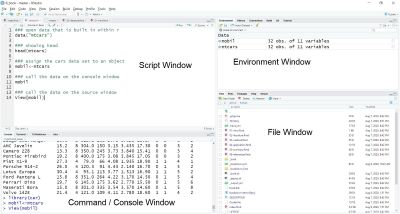
\includegraphics{tampilanR2.JPG}
\caption{\label{fig:unnamed-chunk-1}Tampilan RStudio}
\end{figure}

Secara garis besar, RStudio Memiliki 4(empat) jendela, yaitu script, console, environment dan file. kode yang ada di buku ini harus anda ketik di jendela \emph{`console'}, sementara script merupakan kumpulan kode.

Untuk saat ini, mengetahui nama-nama dari keempat jendela ini sudah cukup. Bagaimana menggunakannya akan diperjelas di bab-bab berikutnya.

\hypertarget{update-r}{%
\section{update R}\label{update-r}}

R merupakan aplikasi yang cukup sering mendapatkan update. Karena itu, anda harus rajin-rajin ngecek update ketika menggunakannya. Jangan lupa juga bahwa anda akan memerlukan kuota internet untuk melakukan update.

Ada banyak cara untuk melakukan update terhadap R, tapi berikut ini akan disampaikan cara tercepat untuk melakukannya dengan menggunakan `console' di RStudio.

pertama, instal paket bernama ``installr'':

\begin{Shaded}
\begin{Highlighting}[]
\KeywordTok{install.packages}\NormalTok{(}\StringTok{"installr"}\NormalTok{)}
\end{Highlighting}
\end{Shaded}

Instalasi paket ini hanya perlu dilakukan pertama kali anda menginstall R. setelah sekali diinstal, paket itu akan selalu ada di komputer anda. Setelah menginstal paket ``installr'', panggil paket tersebut dengan:

\begin{Shaded}
\begin{Highlighting}[]
\KeywordTok{library}\NormalTok{(installr)}
\end{Highlighting}
\end{Shaded}

Fungsi library harus selalu dipanggil ketika akan menggunakan paket tersebut setiap kali anda memulai baru r. Setelah anda memanggil library tersebut, anda tinggal menggunakan fungsi ``updateR()'' pada console.

\begin{Shaded}
\begin{Highlighting}[]
\KeywordTok{updateR}\NormalTok{()}
\end{Highlighting}
\end{Shaded}

Lalu di yes yes saja sampai update selesai.

\hypertarget{intro}{%
\chapter{Memulai dengan R}\label{intro}}

🚧 under construction 🚧

\hypertarget{visualisasi-data}{%
\chapter{Visualisasi Data}\label{visualisasi-data}}

\hypertarget{pendahuluan}{%
\section{Pendahuluan}\label{pendahuluan}}

Visualisasi data yang baik amat diperlukan guna mengkomunikasikan data yang kita miliki kepada orang lain. Visualisasi data dapat berbentuk tabel, grafik garis, grafik batang, dan lain sebagainya. Kali ini kita akan belajar cara melakukan visualisasi data dengan R.

Pada modul ini, kita akan menggunakan paket bernama \texttt{ggplot2} dan paket bernama \texttt{dplyr}. untuk itu, jika belum ada paket ini di komputer anda, maka harus diinstal dengan

Jangan lupa bahwa kita harus terkoneksi dengan internet untuk menginstall paket tersebut. Kita juga harus memanggil paket tersebut dengan

Kita akan menggunakan data yang telah disiapkan di \href{https://imedkrisna.github.io/rbook}{situs buku ini}.

\begin{Shaded}
\begin{Highlighting}[]
\NormalTok{dagang<-}\KeywordTok{read.csv}\NormalTok{(}\KeywordTok{url}\NormalTok{(}\StringTok{"https://imedkrisna.github.io/r/databi.csv"}\NormalTok{))}
\KeywordTok{library}\NormalTok{(lubridate)}
\NormalTok{dagang}\OperatorTok{$}\NormalTok{bulan<-}\KeywordTok{dmy}\NormalTok{(dagang}\OperatorTok{$}\NormalTok{bulan) }\CommentTok{# untuk membuat bulan menjadi waktu}
\KeywordTok{head}\NormalTok{(dagang)}
\end{Highlighting}
\end{Shaded}

\begin{verbatim}
##        bulan  kopi   the rempah tembakau cokelat udang tanilain tekstil   kayu
## 1 2010-01-01 36312 11889  18540     6425  127962 54958   105325  836334 214095
## 2 2010-02-01 36858 11734  16752     4728   67117 60874   125776  814565 241661
## 3 2010-03-01 39535 14239  24954     8512  114329 68049   111998  916195 254687
## 4 2010-04-01 45247 13074  21440    10471   17260 69619   123098  870609 234767
## 5 2010-05-01 60271 12302  25826     6909  127798 63006   119479  888548 229760
## 6 2010-06-01 77593 12322  30163     7282   60956 83919   120270  981359 239067
##    sawit  kimia   logam   alat semen kertas  karet minyak elpiji manufakturlain
## 1 565344 254486  593539 526702  2989 288466 505683 296280     NA        1899732
## 2 805257 256887  548909 581052  6039 298346 631605 325349     NA        1951675
## 3 928524 283782 1002479 683638  8087 350199 773076 246641     NA        2284053
## 4 600508 303844  678313 676969  8881 357734 772325 319986     NA        2314475
## 5 788746 332051  654923 677666  8809 357008 791302 389152     NA        2240443
## 6 864754 237749  681485 670858  5943 345368 780795 234197     NA        2385290
##   tembaga nikel batubara bauksit  crude     gas gascair tambanglain   emas
## 1  263670 39735  1344304   24857 718273 1049665  754473       23575  58107
## 2  446785 34594  1348624   22999 826872  945454  689446       43447  55722
## 3  724134 50842  1520672   42212 913640 1026612  724647       32253  76236
## 4  322333 34815  1399697   33987 866674 1141495  830103       29723 120110
## 5  545442 48632  1277285   33129 903487 1136135  823827       25486 163462
## 6  341779 41563  1510298   43588 885780 1028868  752482       20895 146505
\end{verbatim}

data tersebut merupakan nilai ekspor per bulan Indonesia yang didapat dari \href{https://www.bi.go.id/id/statistik/seki/terkini/eksternal/Contents/Default.aspx}{Statistik Ekonomi dan Keuangan Indonesia (SEKI)}, Bank Indonesia, setelah sebelumnya diolah terlebih dahulu untuk mendapatkan tabel seperti di atas. Data dalam ribu USD.

\hypertarget{grafik}{%
\section{Grafik}\label{grafik}}

Data serial waktu (\emph{time series}) seperti ini memang paling cocok divisualisasikan dengan menggunakan grafik garis. Kita akan mencoba menggambar grafik ekspor biji kopi. kode yang dapat digunakan adalah

\begin{Shaded}
\begin{Highlighting}[]
\NormalTok{grafik<-}\KeywordTok{ggplot}\NormalTok{(dagang,}\KeywordTok{aes}\NormalTok{(}\DataTypeTok{x=}\NormalTok{bulan,}\DataTypeTok{y=}\NormalTok{kopi))}
\NormalTok{grafik<-grafik}\OperatorTok{+}\KeywordTok{geom_line}\NormalTok{()}\OperatorTok{+}\KeywordTok{scale_x_date}\NormalTok{(}\DataTypeTok{date_breaks=}\StringTok{"1 year"}\NormalTok{, }\DataTypeTok{date_labels =} \StringTok{"%Y"}\NormalTok{)}
\KeywordTok{print}\NormalTok{(grafik)}
\end{Highlighting}
\end{Shaded}

\begin{figure}
\centering
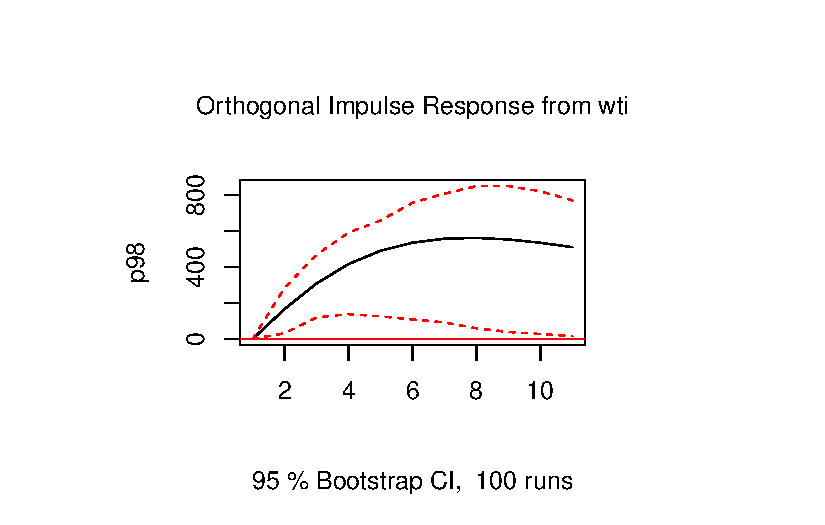
\includegraphics{Modul-belajar-R_files/figure-latex/unnamed-chunk-8-1.pdf}
\caption{\label{fig:unnamed-chunk-8}ekspor bulanan biji kopi}
\end{figure}

Grafik di atas menunjukan perkembangan ekspor bulanan biji kopi Indonesia sejak Januari 2010 sampai Mei 2020.

\hypertarget{latihan}{%
\section{Latihan}\label{latihan}}

Apakah anda dapat menggambar grafik yang sama untuk ekspor kertas? Tuliskan kode-nya di bawah ini

\begin{Shaded}
\begin{Highlighting}[]
\CommentTok{# kode untuk menggambar grafik ekspor kertas}
\end{Highlighting}
\end{Shaded}

\hypertarget{mean-median-dan-modus}{%
\chapter{Mean, Median, dan Modus}\label{mean-median-dan-modus}}

🚧 under construction 🚧

\hypertarget{tes-hipotesis}{%
\chapter{Tes Hipotesis}\label{tes-hipotesis}}

🚧 under construction 🚧

\hypertarget{analisis-regresi}{%
\chapter{Analisis Regresi}\label{analisis-regresi}}

🚧 under construction 🚧

  \bibliography{book.bib}

\end{document}
